%%%%%%%%%%%%%%%%%%%%%%%%%%%%%%%%%%%%%%%%%%%%%%%%
% THIS IS SIGPROC-SP.TEX - VERSION 3.1
% WORKS WITH V3.2SP OF ACM_PROC_ARTICLE-SP.CLS
% APRIL 2009
%
% It is an example file showing how to use the 'acm_proc_article-sp.cls' V3.2SP
% LaTeX2e document class file for Conference Proceedings submissions.
% ----------------------------------------------------------------------------------------------------------------
% This .tex file (and associated .cls V3.2SP) *DOES NOT* produce:
%       1) The Permission Statement
%       2) The Conference (location) Info information
%       3) The Copyright Line with ACM data
%       4) Page numbering
% ---------------------------------------------------------------------------------------------------------------
% It is an example which *does* use the .bib file (from which the .bbl file
% is produced).
% REMEMBER HOWEVER: After having produced the .bbl file,
% and prior to final submission,
% you need to 'insert'  your .bbl file into your source .tex file so as to provide
% ONE 'self-contained' source file.
%
% Questions regarding SIGS should be sent to
% Adrienne Griscti ---> griscti@acm.org
%
% Questions/suggestions regarding the guidelines, .tex and .cls files, etc. to
% Gerald Murray ---> murray@hq.acm.org
%
% For tracking purposes - this is V3.1SP - APRIL 2009
%%%%%%%%%%%%%%%%%%%%%%%%%%%%%%%%%%%%%%%%%%%%%%%

%%%%%%%%%%%%%%%%%%%%%%%%%%%%%%%%%%%%%%%%%%%%%%%
% HSCC 2015 tool paper (6 pages, 10pt, two-column)
% New outline (extended from the old SReach paper)
% Title: SReach: A Model Checking Tool for Stochastic Hybrid Systems
% Abstract
% 1. Introduction
% 2. Probabilistic Bounded Reachability for Hybrid Systems with Parametric Uncertainty
% 	2.1 Hybrid Systems with Parametric Uncertainty
%	2.2 Probabilistic Bounded Reachability
%	2.3 SReach Algorithm
% 3. Probabilistic Bounded Reachability for Stochastic Hybrid Automata
% 	3.1 Stochastic Hybrid Automata
%	3.2 Probabilistic Bounded Reachability
%	3.3 SReach Algorithm
% 		3.3.1 Algorithm 
%		3.3.2 Sampling Method
%		3.3.3 Error Analysis
% 4. Case Studies
%	4.1 Hybrid models with parametric uncertainty
% 		Prostate cancer treatment
%		Atrial Fibrilation
% 		Additional benchmarks
%	4.2 Stochastic hybrid models
%		Killerred Bio system
% 5. Conclusion and Future Work
%%%%%%%%%%%%%%%%%%%%%%%%%%%%%%%%%%%%%%%%%%%%%%%

\documentclass{acm_proc_article-sp}

%%%%%%%%%%%%%%%%%%%%%%%%%%%%%%


\usepackage{caption}

\usepackage{amssymb}
\setcounter{tocdepth}{3}
\usepackage{graphicx}
\usepackage{verbatim}
\usepackage{amsmath}
\usepackage{url}
\usepackage{cite}
\usepackage{listings}
\usepackage{algorithm}
\usepackage{algpseudocode}
\usepackage{bm}
\usepackage{array}
\usepackage{rotating}
\urldef{\mailsa}\path|{alfred.hofmann, ursula.barth, ingrid.haas, frank.holzwarth,|
\urldef{\mailsb}\path|anna.kramer, leonie.kunz, christine.reiss, nicole.sator,|
\urldef{\mailsc}\path|erika.siebert-cole, peter.strasser, lncs}@springer.com|    

\newcommand{\dom}{\mathrm{dom}}
\newcommand{\len}{\mathit{len}}
\newcommand{\poly}{\mathsf{poly}}
\newcommand{\flow}{\mathsf{flow}}
\newcommand{\jump}{\mathsf{jump}}
\newcommand{\inv}{\mathsf{inv}}
\newcommand{\init}{\mathsf{init}}
\newcommand{\guard}{\mathsf{guard}}
\newcommand{\reset}{\mathsf{reset}}
\newcommand{\reach}{\mathsf{Reach}}
\newcommand{\goal}{\mathsf{goal}}
\newcommand{\safe}{\mathsf{safe}}
\newcommand{\p}{\mathsf{P}}
\newcommand{\np}{\mathsf{NP}}
\newcommand{\R}{\mathbb{R}}
\newcommand{\lrf}{\mathcal{L}_{\mathbb{R}_{\mathcal{F}}}}
\newcommand{\citep}{\cite}
\newcommand{\hide}[1]{}
\newcommand{\eg}{{\em e.g.}}
\newcommand{\ie}{{\em i.e.}}
\newcommand{\enforce}{\mathsf{enforce}}

\newtheorem{theorem}{Theorem}[section]
\newtheorem{lemma}[theorem]{Lemma}
\newtheorem{proposition}[theorem]{Proposition}
\newtheorem{corollary}[theorem]{Corollary}


\newenvironment{definition}[1][Definition]{\begin{trivlist}
\item[\hskip \labelsep {\bfseries #1}]}{\end{trivlist}}
\newenvironment{example}[1][Example]{\begin{trivlist}
\item[\hskip \labelsep {\bfseries #1}]}{\end{trivlist}}
\newenvironment{remark}[1][Remark]{\begin{trivlist}
\item[\hskip \labelsep {\bfseries #1}]}{\end{trivlist}}


%%%%%%%%%%%%%%%%%%%%%%%%%%%%%%%

\begin{document}

\title{SReach: A Bounded Model Checker for Stochastic Hybrid Systems}
%\subtitle{SReach: Combining Statistical Tests and Bounded Model Checking}
%
% You need the command \numberofauthors to handle the 'placement
% and alignment' of the authors beneath the title.
%
% For aesthetic reasons, we recommend 'three authors at a time'
% i.e. three 'name/affiliation blocks' be placed beneath the title.
%
% NOTE: You are NOT restricted in how many 'rows' of
% "name/affiliations" may appear. We just ask that you restrict
% the number of 'columns' to three.
%
% Because of the available 'opening page real-estate'
% we ask you to refrain from putting more than six authors
% (two rows with three columns) beneath the article title.
% More than six makes the first-page appear very cluttered indeed.
%
% Use the \alignauthor commands to handle the names
% and affiliations for an 'aesthetic maximum' of six authors.
% Add names, affiliations, addresses for
% the seventh etc. author(s) as the argument for the
% \additionalauthors command.
% These 'additional authors' will be output/set for you
% without further effort on your part as the last section in
% the body of your article BEFORE References or any Appendices.

\numberofauthors{5} 

\author{
% 1st. author
\alignauthor
Qinsi Wang\\
       \affaddr{Computer Science Department}\\
       \affaddr{Carnegie Mellon University}\\
       \affaddr{USA}\\
       \email{qinsiw@cs.cmu.edu}
% 2nd. author
\alignauthor
Paolo Zuliani\\
       \affaddr{School of Computing Science}\\
       \affaddr{Newcastle University}\\
       \affaddr{UK}\\
       \email{paolo.zuliani@ncl.ac.uk}
% 3rd. author
\alignauthor 
Soonho Kong\\
       \affaddr{Computer Science Department}\\
       \affaddr{Carnegie Mellon University}\\
       \affaddr{USA}\\
       \email{soonhok@cs.cmu.edu}
\and  % use '\and' if you need 'another row' of author names
% 4th. author
\alignauthor 
Sicun Gao\\
       \affaddr{Computer Science Department}\\
       \affaddr{Carnegie Mellon University}\\
       \affaddr{USA}\\
       \email{sicung@cs.cmu.edu}
% 5th. author
\alignauthor 
Edmund M. Clarke\\
       \affaddr{Computer Science Department}\\
       \affaddr{Carnegie Mellon University}\\
       \affaddr{USA}\\
       \email{emc@cs.cmu.edu}
}


\maketitle

\begin{abstract}
We present a novel approach solve the probabilistic bounded reachability problem of 
hybrid systems with parameter uncertainty. Standard approaches to this problem require 
numerical solutions for large optimization problems, and become unfeasible for systems 
involving nonlinear dynamics over the reals. Our approach combines randomized 
sampling of probabilistic system parameters, SMT-based bounded reachability analysis, 
and statistical tests. We utilize $\delta-$complete decision procedures 
to solve reachability analysis in a sound way, i.e., we always decide correctly if, for a given
combination of parameters, the system actually reaches the unsafe region.
Compared to standard simulation-based analysis methods, our approach supports 
non-deterministic branching, increases the coverage of simulation, and avoids the
zero-crossing problem. We demonstrate that our method is feasible for general
hybrid systems with parametric uncertainty by applying the implemented tool {\bf SReach} to
a range of nonlinear hybrid systems with parametric uncertainty.

\hide{
We present a novel approach that combines Satisfiability Modulo Theories (SMT) and 
statistical testing to solve the probabilistic bounded reachability problem of 
hybrid systems with parameter uncertainty. That is, we want to find out whether 
a hybrid system with probabilistic system parameters reaches an unsafe region of the
state space within a finite number of steps with a probability greater (or less) than a 
fixed threshold. Standard approaches to this problem require numerical solutions for 
large optimization problems, and become unfeasible for systems involving nonlinear dynamics
over the reals. Our approach solves the reachability problem by combining randomized 
sampling of probabilistic system parameters, SMT-based bounded reachability analysis, 
and statistical tests. In particular, we utilize $\delta-$complete decision procedures 
to solve reachability analysis in a sound way, i.e., we always decide correctly if, for a given
combination of parameters, the system actually reaches the unsafe region (in the opposite case 
we may generate false positives, but this can be controlled by a precision parameter $\delta>0$).
Compared to other simulation-based analysis methods, our approach supports 
non-deterministic branching, increases the coverage of simulation, and avoids the
zero-crossing problem. We demonstrate that our method is feasible for general
hybrid systems with parametric uncertainty by applying the implemented tool {\bf SReach} to
a wide range of nonlinear hybrid systems.}
%to two representative examples - the prostate cancer treatment control and the cardiac system, 
%and further through applications to additional benchmarks.
\vspace{-.7cm}
\end{abstract}
\vspace{-.2cm}
\section{Introduction} 
% motivation for considering shs
% motivation for considering probabilistic reachability
Stochastic hybrid systems (SHSs) are dynamical systems exhibiting discrete, continuous, and stochastic dynamics. Due to their generality, SHSs have been widely used in various areas, including cyber-physical systems, financial decision problems, chemical-physical process control, and biological systems \cite{blom2006stochastic, clarke2011statistical}. The popularity of SHSs in real-world applications motivates researchers to put a significant effort into the analysis methods for this class of systems. One of the elementary questions for the quantitative analysis of SHSs is the probabilistic reachability problem. It is to compute the probability of reaching a certain set of states. The set may represent unsafe states which should be avoided or visited only with some small probability, or dually, good states which should be visited frequently. There are two reasons why this kind of problems catches the researchers' attention. One is that most temporal properties can be reduced to reachability problems, considering the very expressive hybrid modeling framework. The other is that probabilistic state reachability is a hard and challenging problem which is undecidable in general. 

% types of shs
To describe stochastic dynamics, uncertainties have been added to general hybrid systems in a number of different ways. One simplest way replaces some of the system parameters with random variables, resulting in general hybrid automata (GHAs) with parametric uncertainty. Another approach integrates deterministic flows with probabilistic jumps. When state changes forced by continuous dynamics involve discrete random events, we refer to such systems as probabilistic hybrid automata (PHAs) \cite{sproston2000decidable}. When state changes also involve continuous probabilistic events, we call this kind of models stochastic hybrid automata (SHAs) \cite{franzle2011measurability}. Other models describe randomness by substituting deterministic flows with stochastic ones, such as stochastic differential equations (SDEs) \cite{ludwiga1974sde} and stochastic hybrid programs (SHPs) \cite{platzer2011stochastic}, where the random perturbation affects the dynamics continuously. When all such modifications have been applied, the resulting models are called general stochastic hybrid systems (GSHSs) \cite{hu2000towards}. Among these different models, of particular interest for this paper are GHAs with parametric uncertainty and PHAs with additional randomness as both transition probabilities and resets. 


% motivation for considering GHAs with parametric uncertainty
% motivation for considering PHAs 
When modeling real-world systems using hybrid models, parametric uncertainty arises naturally. Although its cause is multifaceted, two factors are critical. On the one hand, probabilistic parameters are needed when the physics controlling the system is known, but some parameters are either not known precisely, or are expected to vary because of individual differences, or may change by the end of the system's operational lifetime. On the other hand, system uncertainty may occur when the model is constructed or learned directly from experimental data. Due to imprecise experimental measurements, the values of system parameters may have ranges of variation with some associated likelihood of occurrence. Clearly, the GHAs with parametric uncertainty are suitable models considering these major causes. Note that, in both cases, we assume that the probability distributions of probabilistic system parameters are known, and it is desired to design models which achieve specified performance for these variations. Another interesting and more expressive class of models is PHAs, which extends hybrid automata \cite{henzinger2000theory} with discrete probability distributions. More precisely, for discrete transitions in a model, instead of making a purely nondeterministic choice over the set of currently enabled jumps, a PHA nondeterministically chooses among the set of recently enabled discrete probability distributions, each of which is defined over a set of transitions. Although randomness is defined to only influence discrete dynamics of the model, PHAs are still very useful and have interesting practical applications \cite{spr2001thesis}. In this paper, we consider a variation of PHAs, where additional randomness of both transition probabilities and resets of some system variables are allowed. In other words, in terms of the randomness on jump probabilities, we mean that the probabilities attached to probabilistic jumps from one mode, instead of obeying to a discrete distribution with predefined constant probabilities, can be expressed by equations involving random variables whose distributions can be either discrete or continuous. This extension is motivated by the fact that some transition probabilities can vary due to factors such as individual differences in real-world systems. When it comes to the randomness of transition resets, we allow that a system variable can be reset to a value obtained according to a known discrete or continuous distribution, instead of being assigned with a fixed value. For example, with this extension, variable $t$ can be updated to any value between $1$ and $5$ with equal probability. %PZ: changed from 2 to 1, otherwise the example does not make sense

{\it {\bf Related Work.}} Analysis approaches for GSHSs are often based on Monte-Carlo simulation \cite{blom2004particle}. Considering the difficulty in dealing with this general case, efforts have been mainly placed on different subclasses. For PHAs, Zhang et al. \cite{zhang2012safety} abstracted the original PHA to a probabilistic automaton (PA), and then used the established Model Checking methods (e.g. PRISM \cite{website:prism}) for the abstract model. Hahn et al. also discussed an abstraction-based method where the given PHA was translated into a $n$-player stochastic game using two different abstraction techniques \cite{hahn2011game}. Another method proposed is a SMT-based bounded Model Checking procedure \cite{franzle2008stochastic}. In \cite{amin2006reachability, abate2007probabilistic, abate2011two, abate2011quantitative}, a similar class of models called discrete-time stochastic hybrid systems (DTSHSs), which is widely used in control theory, was considered. With regard to system analysis, the control problem is to find an optimal control policy that minimizes the probability of reaching unsafe states. Zuliani et al. also mentioned a simulation-based method for model checking DTSHSs against bounded temporal properties \cite{zuliani2010bayesian}. We refer to this method as Statistical Model Checking (StatMC).  Although StatMC does not belong to the class of exhaustive state-space exploration methods, it usually returns results faster than the exhaustive search with a predefined arbitrarily small error bound on the estimated probability. StatMC was recently integrated into UPPAAL \cite{larsen1997uppaal} in order to handle very general networks of SHAs \cite{david2012statistical}. To analyze reachability problems of stochastic hybrid automata (SHAs), a given SHA was first over-approximated by a PHA, and then the verification procedure introduced in \cite{zhang2012safety} was exploited to model check the over-approximating PHA \cite{franzle2011measurability}. Plazter introduced another interesting modeling formalism - stochastic hybrid programs (SHPs) in \cite{platzer2011stochastic}. This formalism is quite expressive on randomness: it takes stochastic differential equations, discrete probabilistic branching, and random assignments to real-valued variables into account. To specify system properties, Platzer proposed a logic called stochastic differential dynamic logic, and then suggested a proof calculus to verify logical properties of SHPs. 


% briefly introduce SReach algorithms
In this paper, we describe our tool {\it SReach} which supports bounded probabilistic reachability analysis for the above two interesting model classes. It combines the recently proposed $\delta$-complete bounded reachability analysis technique \cite{gaodelta} with statistical testing. Our technique saves the virtues of the Satisfiability Modulo Theories (SMT) based Bounded Model Checking for GHAs \cite{cordeiro2012smt, tinelli2012smt}, namely the fully symbolic treatment of hybrid state spaces, while advancing the reasoning power to probabilistic models and requirements. Moreover, by adopting statistical tests, {\it SReach} can place a predefined arbitrarily small error bound on the estimated probability compared to the real value. Comparing to the existing tools introduced in \cite{zhang2012safety, franzle2008stochastic, david2012statistical, website:prism}, besides offering a sound way to analyze nonlinear dynamics within the SHSs, {\it SReach} also supports probabilistic bounded reachability analysis for hybrid systems with parametric uncertainty. Furthermore, for PHAs, {\it SReach} considers a more general and useful formalism where general randomness of transition probabilities and variable resets are allowed. We discuss three biological models - a prostate cancer treatment model, a cardiac atrial fibrillation model, and our synthesized Killerred biological model - to show how {\it SReach} can be used to answer several types of questions including model validation, parameter estimation, and sensitivity analysis. To further demonstrate the feasibility of {\it SReach}, we also present experimental results for additional real-world hybrid systems that are highly nonlinear and nondeterministic.

%Over the last decade, research efforts concerning SHSs are rapidly increasing. At the same time, Model Checking methods and tools for probabilistic systems, such as PRISM \cite{website:prism}, have been proposed. However, results related to the analysis and verification of SHSs are still limited. For instance, analysis approaches for GSHSs are often based on Monte-Carlo simulation \cite{blom2004particle}. Considering the hardness dealing with the general class, efforts have been mainly placed on different subclasses. For PHAs, Zhang et al. abstracted the original PHA to a probabilistic automaton (PA), and then used the established Model Checking methods for the abstracting model \cite{zhang2012safety}. Hahn et al. also discussed an abstraction-based method where the given PHA was translated into a $n$-player stochastic game using two different abstraction techniques \cite{hahn2011game}. Another method proposed is a SMT-based bounded Model Checking procedure \cite{franzle2008stochastic}. \cite{amin2006reachability, abate2007probabilistic, abate2011two, abate2011quantitative} considered a similar class of models that is widely used in the control theory, which is called discrete-time stochastic hybrid systems (DTSHSs). With regard to the system analysis, the control problem concerned can be understood as to find an optimal control policy that minimizes the probability of reaching unsafe states. Zuliani et al. also mentioned a simulation-based method for model checking DTSHSs against bounded temporal properties \cite{zuliani2010bayesian}. We refer to this method as Statistical Model Checking (StatMC).  Although this statistical model checking procedure does not belong to the class of exhaustive state-space exploration methods, it usually returns results faster than the exhaustive search with a predefined arbitrarily small error bound on the estimated probability. StatMC is currently integrated into UPPAAL in order to handle very general networks of SHAs \cite{david2012statistical}. To analyze reachability problems of stochastic hybrid automata (SHAs), in \cite{franzle2011measurability}, a given SHA is firstly over-approximated by a PHA, and then the verification procedure introduced in \cite{zhang2012safety} is exploited to model check the over-approximating PHA. Another interesting work is about stochastic hybrid programs (SHPs) introduced in \cite{platzer2011stochastic}. This formalism is quite expressive on randomness. To specify system properties, Platzer proposed a logic called stochastic differential dynamic logic, and then suggested a proof calculus to verify logical properties of SHPs. 

%Akin to PHAs, DTSHSs comprise nondeterministic as well as discrete probabilistic choices of state transitions. Unlike PHAs, DTSHSs are sampled at discrete time points, use control inputs to model nondeterminism, do not have an explicit notion of symbolic transition guards, and support a more general concept of randomness which can describe discretized stochastic differential equations. With regard to the system analysis, the control problem concerned can be understood as to find an optimal control policy that minimizes the probability of reaching unsafe states. A backward recursive procedure which is also called dynamic programming scheme was then proposed to solve the problem \cite{amin2006reachability, abate2007probabilistic}. Another approach to a very similar problem as above, where a DTSHS model is without nondeterministic control inputs, was presented in \cite{abate2011two}. Comparing to former method where the grid is used to generate and numerically solve a discretized dynamic programming scheme, the latter approach exploits the grid to construct a discrete-time Markov chain (DTMC), and then employs standard model checking procedures for the DTMC. This approach then had been used in \cite{abate2011quantitative} as an analysis procedure for the probabilistic reachability problems in the product of a DTSHS and a B\"{u}chi automaton representing a linear temporal property. Zuliani et al. also mentioned a simulation-based method for model checking DTSHSs against bounded temporal properties \cite{zuliani2010bayesian}. We refer to this method as Statistical Model Checking (StatMC). The main idea of StatMC is to generate enough simulations of the system, record the checking result returned from a trace checker from each simulation, and then use statistical testing and estimation methods to determine, with a predefined degree of confidence, whether the system satisfies the property. Although this statistical model checking procedure does not belong to the class of exhaustive state-space exploration methods, it usually returns results faster than the exhaustive search with a predefined arbitrarily small error bound on the estimated probability. StatMC is currently integrated into UPPAAL in order to handle very general networks of SHAs \cite{david2012statistical}. In \cite{franzle2011measurability}, as an extension of PHAs, stochastic hybrid automata (SHAs) allow continuous probability distributions in the discrete state transitions. With respect to the verification procedure, a given SHA is firstly over-approximated by a PHA via discretizing continuous distributions into discrete ones with the help of additional uncountable nondeterminism. As mentioned, this over-approximation preserves safety properties. For the second step, the verification procedure introduced in \cite{zhang2012safety} is exploited to model check the over-approximating PHA. Another interesting work is about stochastic hybrid programs (SHPs) introduced in \cite{platzer2011stochastic}. This formalism is quite expressive on randomness: it takes stochastic differential equations, discrete probabilistic branching, and random assignments to real-valued variables into account. However, nondeterminism and parallel composition are not considered. To specify system properties, Platzer proposed a logic called stochastic differential dynamic logic, and then suggested a proof calculus to verify logical properties of SHPs. 

The paper starts by introducing the two hybrid modeling formalisms under consideration: GHAs with parametric uncertainty and PHAs with additional randomness in Section 2. Section 3 explains how {\it SReach} encodes stochastic dynamics and combines SMT-based bounded model checking with statistical tests. Case studies and additional experiments are discussed in Section 4. Section 5 concludes the paper.

\section{Models for Stochastic Hybrid Systems}
Before discussing the details of the {\it SReach} algorithm, we first define the two types of formalism that {\it SReach} considers in detail. The first class is GHAs with parametric uncertainty. We follow the definition of GHAs in \cite{henzinger2000theory}, and extend it to consider probabilistic parameters in the following way.
\vspace{-.4cm}
\begin{definition}
\label{def:ha_para}
{\rm(Hybrid Automata with Parametric Uncertainty)} A hybrid automaton with probabilistic parameters is a tuple $H_p = \langle (Q, E), \;V, \;RV, \; \mathsf{Init},\; \mathsf{Flow}, \; \mathsf{Inv}, \; \mathsf{Jump}, \; \Sigma \rangle$, where
\vspace{-.4cm}
\begin{itemize}
\item $(Q, E)$ is a finite directed multigraph. The vertices $Q=\{q_1, \cdots,q_m\}$ is a finite set of discrete modes, and edges in $E$ are control switches.
\vspace{-.2cm}
\item $V = \{ v_1, \cdots, v_n \}$ denotes a finite set of real-valued systems variables, where $n$ is the dimension of $H_p$. We write $\dot{V}$ for the set $\{\dot{v_1}, \cdots, \dot{v_n}\}$ to represent first derivatives of variables during the continuous change, and write $V'$ for the set $\{v_1', \cdots, v_n'\}$ to denote values of variables at the conclusion of the discrete change.
\vspace{-.2cm}
\item $RV = \{ u_1, \cdots, u_k \}$ is a finite set of random variables, where the distribution of $u_i$ is denoted by $P_i$.
\vspace{-.2cm}
\item $\mathsf{Init}$, $\mathsf{Flow}$, and $\mathsf{Inv}$ are labeling functions over each mode $q \in Q$. The initial condition $Init(q)$ is predicate whose free variables are from $V \cup RV$, the invariant condition $Inv(q)$ is a predicate whose free variables are from $V \cup RV$, and the flow condition $Flow(q)$ is a predicate whose free variables are from $V \cup \dot{V} \cup RV$.
\vspace{-.2cm}
\item $\mathsf{Jump}$ is transition labeling function that assigns to each transition $e \in E$ a predicate whose free variables are from $V \cup V' \cup RV$.
\vspace{-.2cm}
\item $\Sigma$ is a finite set of events, and an edge labeling function $event: E \to \Sigma$ assigns to each control switch an event. 
\end{itemize}
\end{definition}
\vspace{-.4cm}
As the other modeling formalism that {\it SReach} currently considers, PHAs with additional randomness are formally defined as follows.
\vspace{-.4cm}
\begin{definition}
\label{def:pha}
{\rm(Probabilistic Hybrid Automata)} A probabilistic hybrid automaton  (with additional randomness) $H$ is a tuple (${\it Q}$, ${\it \bar{q}}$, ${\it V}$, ${\it \left \langle Post_m \right \rangle_{m \in M}}$, $RV$, ${\it Cmds}$) where
\vspace{-.4cm}
\begin{itemize}
\item ${\it Q} := \{ q_1, \cdots, q_n \}$ is a finite set of control modes.
\vspace{-.2cm}
\item ${\it \bar{q}} \subseteq {\it Q}$ is the initial mode.
\vspace{-.2cm}
\item $V = \{ v_1, \cdots, v_k \}$ denotes a finite set of real-numbered systems variables, where $k$ is the dimension of $H$. As mentioned, $\dot{V}$ represents first derivatives of variables, and $V'$ denotes values of variables at the conclusion of the discrete change.
\vspace{-.2cm}
\item ${\it \left \langle Post_q \right \rangle_{q \in Q}}$ indicates continuous timed behaviors on each mode. 
\vspace{-.2cm}
\item $RV$ is a finite set of random variables with known discrete or continuous probability distributions.
\vspace{-.2cm}
\item ${\it Cmds}$ is a finite set of probabilistic guarded commands of the following form: \\
$g \; \rightarrow \; p_1:u_1 \; + \; \cdots \; + \; p_m:u_m$,\\
where $g$ is a predicate representing a transition guard with free variables from $V$, $p_i$ is the transition probability for the $i$th probabilistic choice which can be expressed by an equation involving random variable(s) in $RV$ 
and the $p_i$'s satisfy $\sum_{i=1}^m p_i =1$, and $u_i$ is the corresponding transition function for the $i$th probabilistic choice, whose free variables are from $V \cup V' \cup RV$.
\end{itemize}
\end{definition}
To illustrate the additional randomness allowed on transition probabilities and variable resets, an example probabilistic guarded command can be $x \geq 5 \; \rightarrow \; p_1:(x' = sin(x) + (1-p_1):(x' = p_x))$, where $x$ is a system variable, $p_1 \sim  U(0.2, 0.9)$, and $p_x  \sim  B(0.85)$. This means that, the probability to choose the first transition is not a fixed value, but a random variable obeying to an Uniform distribution. Also, after taking the second transition, $x$ can be assigned to either $1$ with probability $0.85$, or $0$ with $0.15$. In general, for an individual probabilistic guarded command, the transition probabilities can be expressed by equations of one or more novel random variables, as long as values of all transtion probabilities are within $[0, 1]$, and their sum is $1$. Currently, the four primary arithmetic operations are supported. Note that, to preserve the Markov property, only unused random variables can be adopted, so that no dependence between the current probabilistic jump and previous transitions will be introduced. 






\section{SReach algorithm}
The main idea implemented in {\it SReach} is to use a set of random variables to encode all the stochastic information first. In detail, when a hybrid automaton is given, {\it SReach} directly declares each probabilistic system parameter as one random variable with a known distribution. While for a PHA, each probabilistic guarded command $g \rightarrow p_1:u_1 + \cdots + p_m:u_m$ is rewritten by introducing a new random variable $rv$ such that $Pr(rv = i) = p_i$. For example, a probabilistic command $x \geq 1 \to 0.7 : (x' = 1)+ 0.3 :( x' = x)$ will be rewritten as two new guarded commands after introducing a new random variable $r$ whose distribution is $(Pr(r=1)=0.7, Pr(r=2)=0.3)$. One is $x \geq 1 \wedge r = 1 \to x'=1$. The other is $x \geq 1 \wedge r = 2 \to x'=x$. When additional randomness is involved in assigning probabilities for probabilistic transitions or in resetting system variables, addtional random variables are needed. For instance, {\it SReach} can express a probabilistic guarded command as $x \geq 1 \to p_1 : (x' = p_2 )+ (1-p_1) :( x' = x)$, where $p_1$ is a random variable which obeys to an Uniform distribution from 0.6 to 0.85, and $p_2$ is a random variable whose distribution is $N(0,1)$.

After encoding all the stochastic elements using random variables, {\it SReach} samples all random variables according to their probability distributions. For each sampled assignment to these random variables, we obtain a corresponding hybrid automaton by replacing all random variables with assigned values. Then, the bounded model checker for hybrid automata {\it dReach} \cite{gaodelta} is adapted to analyze each obtained hybrid automaton $M_i$, together with the desired precision $\delta$ and the unfolding steps $k$. {\it dReach} returns either unsat or $\delta$-sat for $M_i$ (see Appendix \ref{apndx:dreach} for more on the $\delta$-complete decision procedures). This information
is then used by statistical tests to decide whether to stop or to repeat the procedure. The full procedure is illustrated in Algorithm \ref{fig:sreach}, where $MP$ is a given probabilistic model, and $ST$ indicates which statistical testing method will be used. $Succ$ is used to record the number of $\delta$-sat instances that are returned by {\it dReach}, and $N$ the total of samples generated so far. These two numbers are then the inputs of {\it SReach}'s statistical testing procedure $ST$. Since the full nondeterminism within obtained hybrid automata has been considered when handling the bounded reachability problems, the estimated probabilities computed by {\it SReach} are the maximum probabilities. Also, for a probabilistic hybrid automaton, sampling and fixing all the probabilistic transitions in advance results in an over-approximation of the original probabilistic model. Because the result is an over-approximation, safety properties are preserved. To improve the performance of {\it SReach}, each sampled assignment, together with its corresponding {\it dReach} result, has been recorded for avoiding repeated calls of {\it dReach} with the same sampled assignments. This significantly reduces the total calls to {\it dReach} for PHAs without additional randomness, as the size of sample space is comparatively small. For the example PHA, as shown in Figure \ref{fig:examplepha}, with this improvement, the total checking time for a reachability problem with $k=2$ has been decreased from $11291.31$s for $658$ samples ($17.16$s per sample) to $3295.82$s ($5.01$s per sample). To further improve the performance, a parallel version of {\it SReach} has been implemented, where multiple samples and corresponding hybrid automata are generated, and passed to {\it dReach} simultaneously. Using this parallel version of {\it SReach} on a four-core machine, the running time for the above example PHA has been further decreased to $2119.55s$ for $660$ samples ($3.33$s per sample). 
\begin{figure}
\centering
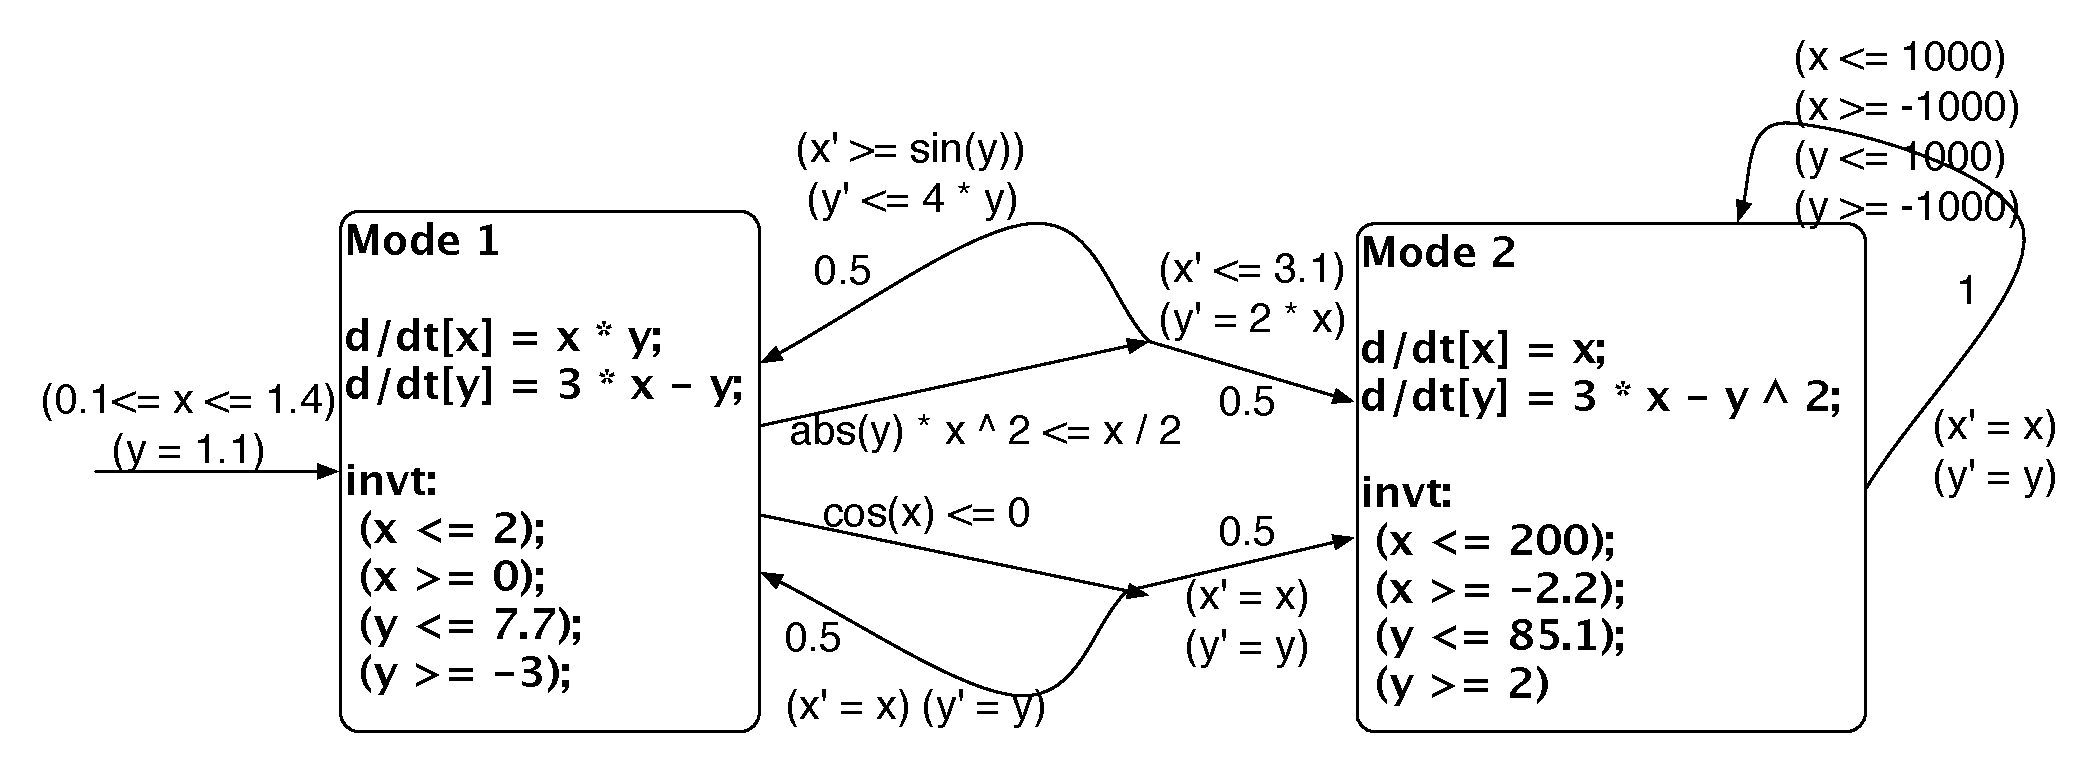
\includegraphics[width=\linewidth]{examplepha}
\caption{An example probabilistic hybrid automaton}
\label{fig:examplepha}
\end{figure}


\begin{algorithm}
  \centering
  \caption{SReach}
  \label{fig:sreach}
  \begin{algorithmic}[1]
    \Function{SReach}{$MP$, $ST$, $\delta$, $k$}
        \State $Succ \gets 0$	\Comment{number of $\delta$-sat samples}
        \State $N \gets 0$	\Comment{total number of samples}
        \State $RV \gets \mathrm{ExtractRV}(MP)$	\Comment{get the RVs from the probabilistic model}
        \Repeat
            \State $S_i \gets \mathrm{Sim}(RV)$		\Comment{sample the parameters}
            \State $M_i \gets \mathrm{Gen}(MP, S_i)$	\Comment{generate a dReach model}
            \State $Res \gets \mathrm{dReach}(M_i, \delta, k)$	\Comment{call dReach}
            \If{$Res$ = $\delta$-sat}
            	%Good
		\State $Succ \gets Succ + 1$
%	  \Else
%	   	%Bad
%		\State $Fail \gets Fail + 1$
	    
	  \EndIf
	\State $N \gets N + 1$
        \Until{$ST.done(Succ, N)$}	\Comment{perform statistical test}\\
        %\State $Est\_prob \gets Succ / N$
	\quad\hspace{0.5ex} \Return $ST.output$
   \EndFunction
  \end{algorithmic}
\end{algorithm}

Currently, {\it SReach} supports a number of hypothesis testing and statistical estimation techniques including: the {Lai's test} \cite{lai1988nearly}, {Bayes factor test} \cite{kass1995bayes}, {Bayes factor test with indifference region} \cite{younes2005verification}, {Sequential probability ratio test (SPRT)}\cite{wald1945sequential}, {Chernoff-Hoeffding bound} \cite{hoeffding1963probability}, {Bayesian Interval Estimation with Beta prior}\cite{zuliani2010bayesian}, and {Direct Sampling}. All methods produce answers to some correctness precision that can be set arbitrarily by the user. See Appendix \ref{apndx:stat} for more details about how these tests can guarantee an arbitrary small error bound between the estimated probability and the real one. With these hypothesis testing methods, {\it SReach} can answer qualitative questions, such as ``Does the model satisfy a given reachability property in $k$ steps with probability greater than a certain threshold?'' While with the above statistical estimation techniques, {\it SReach} can offer answers to quantitative problems. For instance, ``What is the probability that the model satisfies a given reachability property in $k$ steps?''  {\it Sreach} can also handle additional types of interesting problems by encoding them as bounded reachability problems. The {\bf model validation} problem with prior knowledge can be encoded as a bounded reachability question. Expressing prior knowledge about the given model as reachability properties, is there any number of steps $k$ in which the model satisfies a given property? If none exists, the model is incorrect regarding the given prior knowledge. If, for each property, a witness is returned, we can conclude that the model is correct with regard to the prior knowledge. The {\bf parameter estimation} problem can also be encoded as a $k$-step reachability problem. Does there exist a parameter combination for which the model reaches the given goal region in $k$ steps? If so, this parameter combination is potentially a good estimation for system parameters. The goal here is to find an assignment with which all the given goal regions can be reached in a bounded number of steps. Moreover, the {\bf sensitivity analysis} can be conducted by a set of bounded reachability queries as well. Are the results of reachability analysis the same for different possible values of a certain system parameter? If so, the model is insensitive to this parameter with regard to the given prior knowledge.



\section{Experiments}
%\vspace{-.1cm}
Our method is implemented in the open-source tool {\it SReach} (\url{https://github.com/dreal/SReach}). Both a sequential version and a parallel one has been implemented. See Appendix \ref{apndx:usage} for information on using {\it SReach}. All models for the following case studies and additional benchmarks can be found on the tool website. All experiments were conducted on a server with 2* AMD Opteron(tm) Processor 6172 (24 cores) and 32GB RAM, running on Ubuntu 14.04.1 LTS. 12 cores were used. In our experiments we used $0.001$ as the precision for the $\delta$-decision problem; and Bayesian sequential estimation with $0.01$ as the estimation error bound, coverage probability $0.99$, and a uniform prior ($\alpha = \beta = 1$).

{\bf\noindent Prostate cancer treatment.}
%\textit{Model Description}.
This model is a nonlinear hybrid automaton with parametric uncertainty. We modified the model of the intermittent androgen suppression (IAS) therapy in \cite{tanaka2010mathematical} by adding parametric uncertainty. The IAS therapy switches between  treatment-on, and treatment-off with respect to the serum level thresholds of prostate-specific antigen (PSA), namely $r_0$ and $r_1$. As suggested by the clinical trials \cite{bruchovsky2006final}, an effective IAS therapy highly depends on the individual patient. Thus, we modified the model by taking parametric variation caused by personalized differences into account. In detail, according to clinical data from hundreds of patients \cite{bruchovsky2007locally}, we replaced six system parameters with random variables having appropriate (continuous) distributions, including $\alpha_x$ (the proliferation rate of androgen-dependent (AD) cells), $\alpha_y$ (the proliferation rate of androgen-independent (AI) cells), $\beta_x$ (the apoptosis rate of AD cells), $\beta_y$ (the apoptosis rate of AI cells), $m_1$ (the mutation rate from AD to AI cells), and $z_0$ (the normal androgen level). To describe the variations due to individual differences, we assigned $\alpha_x$ to be $U(0.0193, 0.0214)$, $\alpha_y$ to be $U(0.0230, 0.0254)$, $\beta_x$ to be $U(0.0072, 0.0079)$, $\beta_y$ to be $U(0.0160, 0.0176)$, $m_1$ to be $U(0.0000475, 0.0000525) $, and $z_0$ to be $N(30.0, 0.001)$. We used {\it SReach} to estimate the probabilities of preventing the relapse of prostate cancer with three distinct pairs of treatment thresholds (\ie, combinations of $r_0$ and $r_1$).  In the experiments, we chose $k=2$ as the unfolding depth. For each sample generated, {\it SReach} analyzed systems with $41$ variables, and $10$ ODEs. As shown in Table \ref{table:prostate}, the model with thresholds $r_0 = 10$ and $r_1 = 15$ has a probability that approaches 1, indicating that these thresholds may be considered for the general treatment. 
%\vspace{-.5cm}
\begin{table}[th!]
\captionsetup{font=scriptsize}
\centering
    \begin{tabular}{|p{1.1cm} < {\centering}|p{0.65cm} < {\centering}|p{0.65cm} < {\centering}|p{0.65cm} < {\centering}|c|c|c|c|c|}
    \hline
    $(r_0,r_1)$ & Est\_P & \#S\_S & \#T\_S & Avg\_T(s) & Tot\_T(s) \\ \hline
    (5, 10) & 0.496   & 8226      & 16584    & 0.596   & 9892     \\ \hline
    (7, 11) & 0.994  & 335   & 336   & 54.307 & 18247     \\ \hline
    (10, 15) & 0.996  & 240    & 240    & 506.5   & 121560   \\ \hline
    \end{tabular}
    \caption{Results for the prostate cancer treatment model. \#S\_S = number of $\delta$-sat samples, 
\#T\_S = total number of samples, $r_0$ = lower threshold of the serum PSA level, $r_1$ = upper threshold, 
Est\_P = estimated probability of the property,  Avg\_T(s) = average CPU time of each sample in seconds, and Tot\_T(s) = total CPU time for all samples in seconds.}
    \label{table:prostate}
\end{table}
\vspace{-.5cm}

\begin{table}[h!]
\captionsetup{font=scriptsize}
\centering
    \begin{tabular}{|p{1.3cm} < {\centering}|p{1cm} < {\centering}|p{0.7cm} < {\centering}|p{0.7cm} < {\centering}|p{0.7cm} < {\centering}|p{0.7cm} < {\centering}|p{0.7cm} < {\centering}|}
    \hline
    \small{EPI\_TO1}            &\small{EPI\_TO2}         &\small{\#S\_S} & \small{\#T\_S} & \small{Est\_P} & \small{A\_T(s)} & \small{T\_T(s)} \\ \hline
    U(6.1e-3, 7e-3)    & 6              & 240       & 240      & 0.996     & 0.270   & 64.80     \\ \hline
    U(5.5e-3, 5.9e-3)   & 6              & 0         & 240      & 0.004     & 0.042  & 10.08       \\ \hline
    400               & U(0.131, 6)    & 240      & 240      & 0.996     & 0.231  & 55.36      \\ \hline
    400               & U(0.1, 0.129)    & 0         & 240      & 0.004     & 0.038   & 9.15     \\ \hline
    N(400, 1e-4)      & N(6, 1e-4)     & 240       & 240      & 0.996     & 0.091  & 21.87      \\ \hline
    N(5.5e-3, 10e-6) & N(0.11, 10e-5) & 0         & 240      & 0.004     & 0.037  & 8.90      \\ \hline
    \end{tabular}
    \caption {Results for the atrial fibrillation model. \#RVs = number of random variables in the model, \#S\_S = number of $\delta$-sat samples, 
\#T\_S = total number of samples, Est\_P = estimated probability of property,  A\_T(s) = average 
CPU time of each sample in seconds, and T\_T(s) = total CPU time for all samples in seconds.}
    \label{table:cardiac}
\end{table}
\vspace{-.2cm}
{\bf\noindent Atrial Fibrillation.} The minimum resistor model (MRM) reproduces experimentally measured characteristics of human ventricular cell dynamics \cite{bueno2008minimal}. The MRM reduces the complexity of existing models by representing channel gates of different ions with one fast channel, and two slow gates. However, due to this reduction, for most model parameters, it becomes impossible to obtain their values through measurements. With this application, we show that {\it SReach} can also be adapted to estimate parameters of this nonlinear hybrid model with parametric uncertainty. It is to identify appropriate ranges and distributions for model parameters. To illustrate the way in which {\it SReach} is used to conduct parameter estimation, we chose two system parameters - $EPI\_TO1$ and $EPI\_TO2$, and varied their distributions to see which ones of these two system parameters allows the model to present the desired pattern. The model has 4 modes. In the experiments, we chose $3$ as the unfolding depth. For each sample generated, {\it SReach} analyzed systems with $62$ variables, and $24$ ODEs. As in Table \ref{table:cardiac}, when $EPI\_TO1$ is either close to $400$, or between $0.0061$ and $0.007$, and $EPI\_TO2$ is close to $6$, the model can satisfy the given bounded reachability property with a probability very close to $1$. 
%\vspace{-.5cm}
\vspace{-.1cm}

{\bf Synthesized Killerred Model.} Due to the widespread misuse and overuse of antibiotics, drug resistant bacteria now pose significant risks to health, agriculture and the environment. An alternative to conventional antibiotics is phage-based therapy. Our approach to antibiotic resistance is to engineer a temperate phage, Lambda ($\lambda$), with light-activated production of superoxide (SOX). We incorporated the Killerred protein which has been shown to be phototoxic, which can provide another level of controlled bacteria killing \cite{natasa2014killerred}. A probabilistic hybrid automaton for this synthesized Killerred model, as shown in Figure \ref{fig:killerred} in Appendix \ref{apndx:model}, has been constructed. Considering individual differences of bacterial cells and distinct experimental environments, additional randomness on transition probabilities are considered. {\it SReach} was first used to validate this model by estimating the probabilities of killing bacterial cells with different values for $k$, as shown in Table \ref{table:kr01}. We noticed that the probabilities of paths going through mode $6$ to mode $11$ in Figure \ref{fig:killerred} are closing to $0$. To exclude the effect from the sampling of rare events, we increased the probability of entering mode $6$. After this modification, the corresponding probabilities estimated by {\it SReach} still approach $0$. We conclude that it is impossible for this model to enter mode $6$. {\it SReach} was also used to figure out 1) the relation between the time to turn on the light after adding the molecular biology reagent IPTG and the total time to kill bacterial cells (see Table \ref{table:kr02} in Appendix \ref{apndx:exp}), 2) the lower bound for the duration of exposure to light is $3$ (see Table \ref{table:kr03} in Appendix \ref{apndx:exp}), 3) the time to remove IPTG is not sensitive considering whether bacterial cells will be killed, and 4) the upper bound of $SOX_{thres}$ (the necessary concentration of SOX to kill bacterial cells) is $0.6667$. All these findings have been reported to biologists for further checking.

\begin{table}[th!]
\captionsetup{font=scriptsize}
\centering
    \begin{tabular}{|p{1.1cm} < {\centering}|p{0.65cm} < {\centering}|p{0.65cm} < {\centering}|p{0.65cm} < {\centering}|c|c|c|c|c|}
    \hline
    $k$ & Est\_P & \#S\_S & \#T\_S & Avg\_T(s) & Tot\_T(s) \\ \hline
    5 &  0.544  & 8951     &  16452   & 0.074   & 1219.38     \\ \hline
    6 & 0.247  & 3045   & 12336   & 0.969 & 11957.12     \\ \hline
    7 & 0.096  & 559    & 5808    & 5.470   & 31770.36   \\ \hline
    8 & 0.004  & 0      & 240    & 0.004  & 0.88     \\ \hline
    9 & 0.004  & 0   & 240   & 0.012 & 2.97     \\ \hline
    10 & 0.004  & 0    & 240    & 0.013   & 3.18   \\ \hline
    \end{tabular}
    \caption{Results for the killerred model. \#S\_S = number of $\delta$-sat samples, 
\#T\_S = total number of samples, $r_0$ = lower threshold of the serum PSA level, $r_1$ = upper threshold, 
Est\_P = estimated probability of the property,  Avg\_T(s) = average CPU time of each sample in seconds, and Tot\_T(s) = total CPU time for all samples in seconds.}
    \label{table:kr01}
\end{table}
\vspace{-.3cm}


{\bf Additional benchmarks.} To further demonstrate the feasibility of {\it SReach}, we also applied it to additional benchmarks including hybrid systems with parametric uncertainty, PHAs, and PHAs with additional randomness. Appendix \ref{apndx:exp} shows the results of these experiments. Moreover, the detailed description of some of the additional benchmarks and above case studies are presented in Appendix \ref{apndx:model}.

\vspace{-.2cm}
\section{Conclusions and future work}
We present a probabilistic reachability analysis tool. The tool combines the $\delta$-decision 
procedure \cite{gao2013dreal, gao2013satisfiability, gaodelta} and statistical testing techniques. 
It supports bounded reachability analysis for hybrid systems with parametric 
uncertainty and probabilistic hybrid automata with additional randomness. This tool was used for the bounded reachability analysis of three representative examples - a prostate 
cancer treatment control, a cardiac model, and a synthesized Killerred model - which are currently out of the reach of other formal (SMT-based) tools. In the near future, we plan to extend support for more general stochastic hybrid models 
that include probabilistic jumps with continuous distributions, and stochastic differential equations.

\bibliography{ref}{}
\bibliographystyle{abbrv}

%%%%%%%%%%%%%%%%%%%%
\newpage
\appendix


\section{Statistical tests}\label{apndx:stat}
In this section we briefly describe the statistical techniques implemented in {\bf SReach}.
To deal with qualitative questions, {\bf SReach} supports the following hypothesis testing methods.

\textit{Lai's test} \cite{lai1988nearly}.
As a simple class of sequential tests, it tests the one-sided composite hypotheses $H_0: \; \theta \leq \theta_0$ versus $H_1:\; \theta \geq \theta_1$ for the natural parameter $\theta$ of an exponential family of distributions under the $0-1$ loss and cost $c$ per observation. \cite{lai1988nearly} shows that these tests have nearly optimal frequentist properties and also provide approximate Bayes solutions with respect to a large class of priors. 

\textit{Bayes factor test} \cite{kass1995bayes}.
The use of Bayes factors is a Bayesian alternative to classical hypothesis testing. It is based on the Bayes theorem. Hypothesis testing with Bayes factors is more robust than frequentist hypothesis testing, as the Bayesian form avoids model selection bias, evaluates evidence in favor the null hypothesis, includes model uncertainty, and allows non-nested models to be compared. Also, frequentist significance tests become biased in favor of rejecting the null hypothesis with sufficiently large sample size. 

\textit{Bayes factor test with indifference region}. 
A hypothesis test has ideal performance if the probability of the Type-I error (respectively, Type-II error) is exactly $\alpha$ (respectively, $\beta$). However, these requirements make it impossible to ensure a low probability for both types of errors simultaneously (see \cite{younes2005verification} for details). A solution is to use an indifference region. The indifference region indicates the distance between two hypotheses, which is set to separate the two hypotheses.

\textit{Sequential probability ratio test (SPRT)} \cite{wald1945sequential}. 
The SPRT considers a simple hypothesis $H_0:\;\theta = \theta_0$ against a simple alternative $H_1:\;\theta = \theta_1$. With the critical region $\Lambda_n$ and two thresholds $A$, and $B$, SPRT decides that $H_0$ is true and stops when $\Lambda_n < A$. It decides that $H_1$ is true and terminates if $\Lambda_n > B$. If $A\; < \Lambda_n < B$, it will collect another observation to obtain a new critical region $\Lambda_{n+1}$. The SPRT is optimal, among all sequential tests, in the sense that it minimizes the average sample size.

To offer quantitative answers, {\bf SReach} also supports estimation procedures as below.

\textit{Chernoff-Hoeffding bound} \cite{hoeffding1963probability}. To estimate the mean $p$ of a (bounded) 
random variable, given a precision $\delta'$ and coverage probability $\alpha$, the Chernoff-Hoeffding bound 
computes a value $p'$ such that $|p' \; - \; p| \le \delta'$ with probability at least $\alpha$.

\textit{Bayesian Interval Estimation with Beta prior} \cite{zuliani2010bayesian}. This method estimates $p$, the unknown probability that a random sampled model satisfies a specified reachability property. 
The estimate will be in the form of a confidence interval, containing $p$ with an arbitrary high probability.  \cite{zuliani2010bayesian} assumes that the unknown $p$ is given by a random variable, whose density is called the prior density, and focuses on Beta priors. %It has been showed that, with this Bayesian interval estimation method, the probability of giving a wrong answer is arbitrarily small, and speed of obtaining an answer is higher than the sequential hypothesis testing.

\textit{Direct sampling}. Given $N$ as the number of samples to be sampled, the direct sampling method estimates the mean of $p$ of a (bounded) random variable. According to the central limit thoerem \cite{durrett2010probability}, the error $\epsilon$ with a confidence $c$ between the real probability $p$ and the estimated $\hat{p}$ is bounded: \\
$\epsilon  =  \phi^{-1}\left ( \frac{c + 1}{2} \right ) \sqrt{\frac{p(1-p)}{N}}$\\
where $\phi(x) = \frac{1}{\sqrt{2\pi}} \int_{-x}^{x} e^{-t^2 / 2}dt$. That is, as $N$ goes to $\infty$, the estimated probability approaches to the real one.

\section{$\delta$-Decisions for Hybrid Models}\label{apndx:dreach}
The reachability problems of hybrid automata can be encoded using a first-order language $\lrf$ over the reals,
which allows the use of a wide range of real functions including nonlinear ODEs.
Then, $\delta$-complete decision procedures are used to find solutions to these formulas to synthesize
parameters.
\begin{definition}[$\lrf$-Formulas]
Let $\mathcal{F}$ be a collection of computable real functions. We define:
\begin{align*}
t& := x \; | \; f(t(\vec x)), \mbox{ where }f\in \mathcal{F} \mbox{ (constants are 0-ary functions)};\\
\varphi& := t(\vec x)> 0 \; | \; t(\vec x)\geq 0 \; | \; \varphi\wedge\varphi
\; | \; \varphi\vee\varphi \; | \; \exists x_i\varphi \; |\; \forall x_i\varphi.
\end{align*}
\end{definition}
By computable real function we mean Type 2 computable, which informally requires that a (real)
function can be algorithmically evaluated with arbitrary accuracy. Since in general
$\lrf$ formulas are undecidable, the decision problem needs to be relaxed. In particular, for
any $\lrf$ formula $\phi$ and any rational $\delta >0$ one can obtain a $\delta$-weakening
formula $\phi^\delta$ from $\phi$ by substituting the atoms $t > 0$ with $t > -\delta$ (and
similarly for $t \geq 0$). Obviously, $\phi$ implies $\phi^\delta$, but not the {\em vice versa}.
Now, the $\delta$-decision problem is deciding correctly whether:
\begin{itemize}
\item $\phi$ is false ($\mathsf{unsat}$);
\item $\phi^\delta$ is true ($\delta$-$\mathsf{sat}$).
\end{itemize}
If both cases are true, then either decision is correct. More details on algorithms ($\delta$-{\em complete} decision procedures) for solving $\delta$-decision problems for $\lrf$ and for ODEs can be found in \cite{gao2013satisfiability, gao2013dreal, gaodelta}.

Now we state the encoding for hybrid models. Hybrid automata generalize finite-state
automata by permitting continuous time flow in each discrete mode.
Also, in each mode an {\em invariant} must be satisfied by the flow, and mode switches are controlled
by {\em jump} conditions.
\begin{definition}[$\lrf$-Representations of Hybrid Automata]\label{lrf-definition}
A hybrid\\ automaton in $\lrf$-representation is a tuple
\begin{multline*}
H = \langle X, Q, \{{\flow}_q(\vec x, \vec y, t): q\in Q\},\{\inv_q(\vec x): q\in Q\},\\
\{\jump_{q\rightarrow q'}(\vec x, \vec y): q,q'\in Q\},\{\init_q(\vec x): q\in Q\}\rangle
\end{multline*}
where $X\subseteq \mathbb{R}^n$ for some $n\in \mathbb{N}$, $Q=\{q_1,...,q_m\}$ is a finite set of modes, and the other components are finite sets of quantifier-free $\lrf$-formulas.
\end{definition}

We now show the encoding of bounded reachability, which is used for encoding the parameter synthesis
problem. We want to decide whether a given
hybrid system reaches a particular region of its state space after following a (bounded) number
of discrete transitions, \ie, jumps. First, we need to define auxiliary formulas used
for ensuring that a particular mode is picked at a certain step.
\begin{definition}
Let $Q = \{q_1,...,q_m\}$ be a set of modes. For any $q\in Q$, and $i\in\mathbb{N}$, use $b_{q}^i$ to represent a Boolean variable. We now define
$$\enforce_Q(q,i) = b^i_{q} \wedge \bigwedge_{p\in Q\setminus\{q\}}\neg b^{i}_{p}$$
$$\enforce_Q(q, q',i) = b^{i}_{q}\wedge \neg b^{i+1}_{q'} \wedge \bigwedge_{p\in Q\setminus\{q\}} \neg b^i_{p} \wedge \bigwedge_{p'\in Q\setminus\{q'\}} \neg b^{i+1}_{p'}$$
We omit the subscript $Q$ when the context is clear.\end{definition}
We can now define the following formula that checks whether a {\em goal} region of the automaton
state space is reachable after exactly $k$ discrete transitions. We first state
the simpler case of a hybrid system without invariants.
\begin{definition}[$k$-Step Reachability, Invariant-Free Case]
Suppose $H$ is an invariant-free hybrid automaton, $U$ a subset of its state space represented by $\goal$,
and $M>0$. \\The formula $\reach_{H,U}(k,M)$ is defined as:
\begin{eqnarray*}
%\reach^{k,M}(H,U) &:=&
& &\exists^X \vec x_{0} \exists^X\vec x_{0}^t\cdots \exists^X \vec x_{k}\exists^X\vec x_{k}^t\exists^{[0,M]}t_0\cdots \exists^{[0,M]}t_k.\\
& &\bigvee_{q\in Q} \Big(\init_{q}(\vec x_{0})\wedge \flow_{q}(\vec x_{0}, \vec x_{0}^t, t_0)\wedge \enforce(q,0)\Big)\\%\wedge (b_{q_i}\wedge \bigwedge_{q\neq q_i} \neg b_{q})
\wedge & & \bigwedge_{i=0}^{k-1}\bigg( \bigvee_{q, q'\in Q} \Big(\jump_{q\rightarrow q'}(\vec x_{i}^t, \vec x_{i+1})\wedge \enforce(q,q',i)\\
& & \hspace{1.1cm}\wedge\flow_{q'}(\vec x_{i+1}, \vec x_{i+1}^t, t_{i+1}) \wedge \enforce(q',i+1)\Big)\bigg)\\
\wedge & &\bigvee_{q\in Q} (\goal_q(\vec x_{k}^t)\wedge \enforce(q,k))
\end{eqnarray*}
where $\exists^X x$ is a shorthand for $\exists x\in X$.
\end{definition}
Intuitively, the trajectories start with some initial state satisfying $\init_q(\vec x_{0})$ for some $q$.
Then, in each step the trajectory follows $\flow_q(\vec x_{i}, \vec x_{i}^t, t)$ and makes a continuous flow from $\vec x_i$ to $\vec x_i^t$ after time $t$. When the automaton makes a $\jump$ from mode $q'$ to $q$, it resets variables following $\jump_{q'\rightarrow q}(\vec x_{k}^t, \vec x_{k+1})$. The auxiliary $\enforce$ formulas ensure that picking $\jump_{q\rightarrow q'}$ in the $i$-the step enforces picking $\flow_q'$ in the $(i+1)$-th step.
When the invariants are not trivial, we need to ensure that for all the time points along a continuous flow, the invariant condition holds. We need to universally quantify over time, and the encoding is as follows:
\begin{definition}[$k$-Step Reachability, Nontrivial Invariant]\label{br2}
Suppose $H$ contains invariants, and $U$ is a subset of the state space represented by $\goal$. The $\lrf$-formula $\reach_{H,U}(k,M)$ is defined as:
\begin{eqnarray*}
& &\exists^X \vec x_{0} \exists^X\vec x_{0}^t\cdots \exists^X \vec x_{k}\exists^X\vec x_{k}^t \exists^{[0,M]}t_0\cdots \exists^{[0,M]}t_k.\\
& &\bigvee_{q\in Q} \Big(\init_{q}(\vec x_{0})\wedge \flow_{q}(\vec x_{0}, \vec x_{0}^t, t_0)\wedge \enforce(q,0)\\
& &\hspace{1.1cm} \wedge \forall^{[0,t_0]}t\forall^X\vec x\;(\flow_{q}(\vec x_{0}, \vec x, t)\rightarrow \inv_{q}(\vec x))\Big) \\
\wedge & &\bigwedge_{i=0}^{k-1}\bigg( \bigvee_{q, q'\in Q} \Big(\jump_{q\rightarrow q'}(\vec
x_{i}^t, \vec x_{i+1})\wedge \flow_{q'}(\vec x_{i+1}, \vec x_{i+1}^t, t_{i+1})\\
& &\hspace{1.1cm} \wedge \enforce(q,q',i) \wedge\enforce(q',i+1)\\
& &\hspace{1.1cm} \wedge \forall^{[0,t_{i+1}]}t\forall^X\vec x\;(\flow_{q'}(\vec x_{i+1}, \vec x,
t)\rightarrow \inv_{q'}(\vec x)) )\Big)\bigg)\\
\wedge & &\bigvee_{q\in Q} (\goal_q(\vec x_{k}^t)\wedge \enforce(q,k)).
\end{eqnarray*}
\end{definition}
The extra universal quantifier for each continuous flow expresses the requirement that for all the time points between the initial and ending time point ($t\in[0,t_i+1]$) in a flow, the continuous variables $\vec x$ must take values that satisfy the invariant conditions $\inv_q(\vec x)$.


\section{The SReach tool}\label{apndx:usage}
\subsection{Input format}
The inputs to our {\it SReach} tool are descriptions of (stochastic) hybrid automata with random variables (representing the probabilistic system parameters, and probabilistic jumps), and the reachability property to be checked. Following roughly the same format as the above definition of (stochastic) hybrid automata, and adding the declarations of random variables, the description of an automaton is as follows.

{\bf Preprocessor.} We can use the C language syntax to define constants and macros. 

{\bf Variable declaration.} For a random variable, the declaration specifies its distribution and name. Variables which are not random variables are required to be declared within bounds. 

{\bf (Probabilistic) Hybrid automaton.} A (probabilistic) hybrid automaton is represented by a set of modes. Within each mode declaration, we can specify statements for the mode invariant(s), flow function(s), and (probabilistic) jump condition(s). For a mode invariant, we can give any logic formula of the variables. A flow function is expressed by an ODE.  As for a nonprobabilistic jump condition, it is written as 
\vspace{-0.4cm}
\begin{verbatim} 
<logic_formula1>  ==> 
            @<target_mode>  <logic_formula2>,
\end{verbatim}
\vspace{-0.4cm}
where the first logic formula is given as the guard of the jump, and the second one specifies the reset condition after the jump. While for a probabilistic jump condition, we need an extra constraint to express the stochastic choice, which is of the following form
\vspace{-0.4cm}
\begin{verbatim}
(and <logic_formula1> <stochastic choice>)  ==> 
            @<target_mode>  <logic_formula2>,
\end{verbatim}
\vspace{-0.4cm}
where the stochastic choice is a formula indicating which probabilistic transition will be chosen for this jump.

{\bf Initial conditions and Goals.} Following the declaration of modes, we can declare one initial mode with corresponding conditions, and the reachability properties in the end.

\noindent\textit{Example 1}. The following is an example input file for a hybrid automaton with parametric uncertainty. Currently, users can specify random variables (representing certain system parameters) with Bernoulli distribution (B), Uniform distribution (U), Gaussian distribution (N), Exponential distribution (E), and general Discrete distribution with given possible values and corresponding probabilities (DD). 
\lstset{basicstyle=\ttfamily\small, numbers=left, breaklines=true }
\begin{lstlisting}
#define pi 3.1416
N(1,0.1) mu1;
U(10,15) thro;
E(0.49) theta1;
B(0.75) xinit;
DD(0:0.7, 1:0.3) mu2;
[0,5] x;
[0,3] time;
{ mode 1; 
  invt:
         (x<=1.5);
         (x>=0);
  flow:
	 d/dt[x]=thro*(1/(theta1*sqrt(2*pi)))
	          *exp(0-((x-mu1+mu2)^2)/(2*theta1^2));
  jump:
        (x>=(thre1+5))==>@2(x'=x);
}
init:
@1	(x=xinit);
goal:
@4	(x>=50);
\end{lstlisting}

\noindent\textit{Example 2}.  This example demonstrates the format of the input file for a probabilistic hybrid automaton. Note that, unlike the notations of declarations of random variables representing system parameters, declarations of random variables used to express transition probabilities for probabilistic jumps start with a prefix $j$.
\lstset{basicstyle=\ttfamily\small, numbers=left, breaklines=true }
\begin{lstlisting}
jU(0.7, 0.9) pjumprv;
DD(1:pjumprv, 2:(1 - pjumprv)) pjump1;
DD(1:0.3, 2:0.7) pjump2;
[-1000, 1000] x;
[-1000, 1000] y;
[0, 3] time;

{ mode 1;

  invt:
        (x <= 2);
        (x >= 0);
	(y <= 7.7);
	(y >= -3);
  flow:
        d/dt[x] = x * y;
        d/dt[y] = 3 * x - y;
  jump:
        (and (abs(y) * x ^ 2 <= x / 2) (pjump1 = 1)) ==> @1 (and (x' >= sin(y)) (y' <= 4 * y));
	(and (abs(y) * x ^ 2 <= x / 2) (pjump1 = 2)) ==> @2 (and (x' <= 3.1) (y' = 2 * x));
	(and (cos(x) <= 0) (pjump2 = 1)) ==> @2 (and (x' = x) (y' = y));
	(and (cos(x) <= 0) (pjump2 = 2)) ==> @1 (and (x' = x) (y' = y));
}

{
  mode 2;
  invt:
        (x <= 200);
        (x >= -2.2);
	(y <= 85.1);
	(y >= 2);
  flow:
        d/dt[x] = x;
        d/dt[y] = 3 * x - y ^ 2;
  jump:
        (and (x <= 1000) (x >= -1000) (y <= 1000) (y >= -1000)) ==> @2 (and (x' = x) (y' = y));
}
init:
@1	(and (x >= 0.1) (x <= 1.4) (y = 1.1));

goal:
@2	(and (x >= -10) (y >= -10));
\end{lstlisting}


\subsection{Command line}
{\it SReach} offers two choices. It can be run sequentially by typing
\vspace{-0.4cm}
\begin{verbatim} 
sreach_sq <statistical_testing_option> <filename> 
		<dReach> <k> <delta>,
\end{verbatim} 
\vspace{-0.4cm}
or in parallel by 
\vspace{-0.4cm}
\begin{verbatim} 
sreach_para <statistical_testing_option> <filename> 
		<dReach> <k> <delta>,
\end{verbatim} 
\vspace{-0.4cm}
where:
\begin{itemize}
\item \verb+statistical_testing_option+ is a text file containing a sequence of test specifications. We will introduce the usages of statistical testing options in the following part;
\item \verb+filename+ is a .pdrh file describing the model of a hybrid system with probabilistic system parameters. It is of the input format described in last sub-section;
\item \verb+dReach+ is a tool for bounded reachability analysis of hybrid systems based on dReal;
\item \verb+k+ is the number of steps of the model that the tool will explore; and
\item \verb+delta+ is the precision for the $\delta$-decision problem.
\end{itemize}

\subsection{Statistical testing options}

{\it SReach} can be used with different statistical testing methods through the following specifications.

\textit {Lai's test}: \verb+Lai <theta> <cost_per_sample>+, where \verb+theta+ indicates the probability threshold.
 
\textit {Bayes factor test}: \verb+BFT <theta> <T> <alpha> <beta>+,
where \verb+theta+ is a probability threshold satisfying \verb+0 < theta < 1+, \verb+T+ is a ratio threshold satisfying \verb+T > 1+, and \verb+alpha+, and \verb+beta+ are beta prior parameters.

\textit {BFT with indifference region}: \\ \verb+BFTI <theta> <T> <alpha> <beta> <delta>+,
where, besides the parameters used in the above Bayes factor test, \verb+delta+ is given to create the indifference region - [$p_0$, $p_1$], where $p_0$ = \verb+theta+ - \verb+delta+ and $p_1$ = \verb+theta+  + \verb+delta+.  Now, it tests $H_0 :\; p \ge p_0$ against $H_1:\; p \le p_1$ .

\textit {Sequential probability ratio test (SPRT)}: \\ \verb+SPRT <theta> <T> <delta>+.

\textit {Chernoff-Hoeffding bound}:\\ \verb+CHB <delta1> <coverage_probability>+,
where \verb+delta1+ is the given precision, and \verb+coverage_probability+ indicates the confidence.

\textit {Bayesian Interval Estimation with Beta prior}: \\ \verb+BEST <delta1> <coverage_probability> <alpha> <beta>+.

\textit {Direct/Na\"{i}ve Sampling}: \verb+NSAM <num_of_samples>+.



\section{Model description}\label{apndx:model}

\textbf{\textit{Atrial Fibrillation.}} The model has four discrete control locations, four state variables, and nonlinear ODEs. A typical set of ODEs in the model is:
\begin{eqnarray*}
\frac{du}{dt} &=& e + (u-\theta_v)(u_u-u ) v g_{fi} + wsg_{si}-g_{so}(u)\\
\frac{ds}{dt} &=& \displaystyle\frac{g_{s2}}{(1+\exp(-2k(u-us)))} -  g_{s2}s\\
\frac{dv}{dt} &=& -g_v^+\cdot v \hspace{1cm} \frac{dw}{dt} = -g_w^+\cdot w
\end{eqnarray*}
The exponential term on the right-hand side of the ODE is the sigmoid function, which often appears in modelling biological switches.

\textbf{\textit{Electronic Oscillator.}} The 3dOsc model represents an electronic oscillator model that contains nonlinear ODEs such as the following.
\begin{eqnarray*}
\frac{dx}{dt} &=& - ax \cdot sin(\omega_1 \cdot \tau)\\
\frac{dy}{dt} &=& - ay \cdot sin( (\omega_1 + c_1) \cdot \tau) \cdot sin(\omega_2)\cdot 2\\
\frac{dz}{dt} &=& - az \cdot sin( (\omega_2 + c_2) \cdot \tau) \cdot cos(\omega_1)\cdot 2\\
\frac{\omega_1}{dt} &=& - c_3\cdot \omega_1\ \ \ \frac{\omega_2}{dt} = -c_4\cdot\omega_2\ \ \ \frac{d\tau}{dt} = 1
\end{eqnarray*}

\textbf{\textit{Quadcopter Control.}} We developed a model that contains the full dynamics of a quadcopter. We use the model to solve control problems by answering reachability questions. A typical set of the differential equations are the following.
\begin{eqnarray*}
\frac{\mathrm{d}\omega_x}{\mathrm{d}t} &=& L\cdot k\cdot (\omega_1^2 - \omega_3^2)(1/I_{xx})-(I_{yy} - I_{zz})\omega_y\omega_z/I_{xx}\\
\frac{\mathrm{d}\omega_y}{\mathrm{d}t} &=& L\cdot k\cdot(\omega_2^2 - \omega_4^2)(1/I_{yy})-(I_{zz} - I_{xx})\omega_x\omega_z/I_{yy}\\
\frac{\mathrm{d}\omega_z}{\mathrm{d}t} &=& b\cdot(\omega_1^2 - \omega_2^2 + \omega_3^2 - \omega_4^2)(1/I_{zz})-(I_{xx} - I_{yy})\omega_x\omega_y/I_{zz}\\
\frac{\mathrm{d}\phi}{\mathrm{d}t} &=& \omega_x + \displaystyle{\frac{\sin\left(\phi\right) \sin\left(\theta\right)}{{\left(\frac{\sin\left(\phi\right)^{2} \cos\left(\theta\right)}{\cos\left(\phi\right)} + \cos\left(\phi\right) \cos\left(\theta\right)\right)} \cos\left(\phi\right)}}\omega_y\\
& &+\displaystyle\frac{\sin\left(\theta\right)}{\frac{\sin\left(\phi\right)^{2} \cos\left(\theta\right)}{\cos\left(\phi\right)} + \cos\left(\phi\right) \cos\left(\theta\right)}\omega_z\\
\frac{\mathrm{d}\theta}{\mathrm{d}t} &=& -(\displaystyle\frac{\sin\left(\phi\right)^{2} \cos\left(\theta\right)}{{\left(\frac{\sin\left(\phi\right)^{2} \cos\left(\theta\right)}{\cos\left(\phi\right)}\omega_y + \cos\left(\phi\right) \cos\left(\theta\right)\right)} \cos\left(\phi\right)^{2}}\\
& &+ \frac{1}{\cos\left(\phi\right)})\omega_y -\displaystyle\frac{\sin\left(\phi\right) \cos\left(\theta\right)}{{\left(\frac{\sin\left(\phi\right)^{2} \cos\left(\theta\right)}{\cos\left(\phi\right)} + \cos\left(\phi\right) \cos\left(\theta\right)\right)} \cos\left(\phi\right)}\omega_z \\
\frac{\mathrm{d}\psi}{\mathrm{d}t} &=& \displaystyle\frac{\sin\left(\phi\right)}{{\left(\frac{\sin\left(\phi\right)^{2} \cos\left(\theta\right)}{\cos\left(\phi\right)} + \cos\left(\phi\right) \cos\left(\theta\right)\right)} \cos\left(\phi\right)}\omega_y\\
& &+ \displaystyle\frac{1}{\frac{\sin\left(\phi\right)^{2} \cos\left(\theta\right)}{\cos\left(\phi\right)} + \cos\left(\phi\right) \cos\left(\theta\right)}\omega_z\\
\frac{\mathrm{d}{xp}}{\mathrm{d}t} &=& (1/m)(\sin(\theta)\sin(\psi)k(\omega_1^2 + \omega_2^2 +\omega_3^2+\omega_4^2) - k\cdot d\cdot{xp})\\
\frac{\mathrm{d}{yp}}{\mathrm{d}t} &=& (1/m)(-\cos(\psi)\sin(\theta)k(\omega_1^2 + \omega_2^2 +\omega_3^2+\omega_4^2) - k\cdot d\cdot{yp})\\
\frac{\mathrm{d}{zp}}{\mathrm{d}t} &=& (1/m)(-g-\cos(\theta)k(\omega_1^2 + \omega_2^2 +\omega_3^2+\omega_4^2) - k\cdot d\cdot{zp}\\
\frac{\mathrm{d}x}{\mathrm{d}t} &=& {xp}, \frac{\mathrm{d}y}{\mathrm{d}t} = {yp}, \frac{\mathrm{d}z}{\mathrm{d}t} = {zp}
\end{eqnarray*}

\textbf{\textit{Prostate Cancer Treatment.}} The Prostate Cancer Treatment model exhibits more nonlinear ODEs. 
\begin{eqnarray*}
\frac{dx}{dt} &=& (\alpha_x
(k_1+(1-k_1)\frac{z}{z+k_2}-\beta_x( (1-k_3)\frac{z}{z+k_4}+k_3))\\
& &- m_1(1-\frac{z}{z_0}))x + c_1 x\\
\frac{dy}{dt} &=& m_1(1-\frac{z}{z_0})x+(\alpha_y (1- d\frac{z}{z_0}) - \beta_y)y+c_2y\\
\frac{dz}{dt} &=& \frac{-z}{\tau} + c_3z\\
\frac{dv}{dt} &=& (\alpha_x
(k_1+(1-k_1)\frac{z}{z+k_2}-\beta_x(k_3+(1-k_3)\frac{z}{z+k_4}))\\
& &- m_1(1-\frac{z}{z_0}))x + c_1 x + m_1(1-\frac{z}{z_0})x+(\alpha_y (1- d\frac{z}{z_0})\\
& &- \beta_y)y+c_2y
\end{eqnarray*}

\begin{figure*}[ht]
\centering
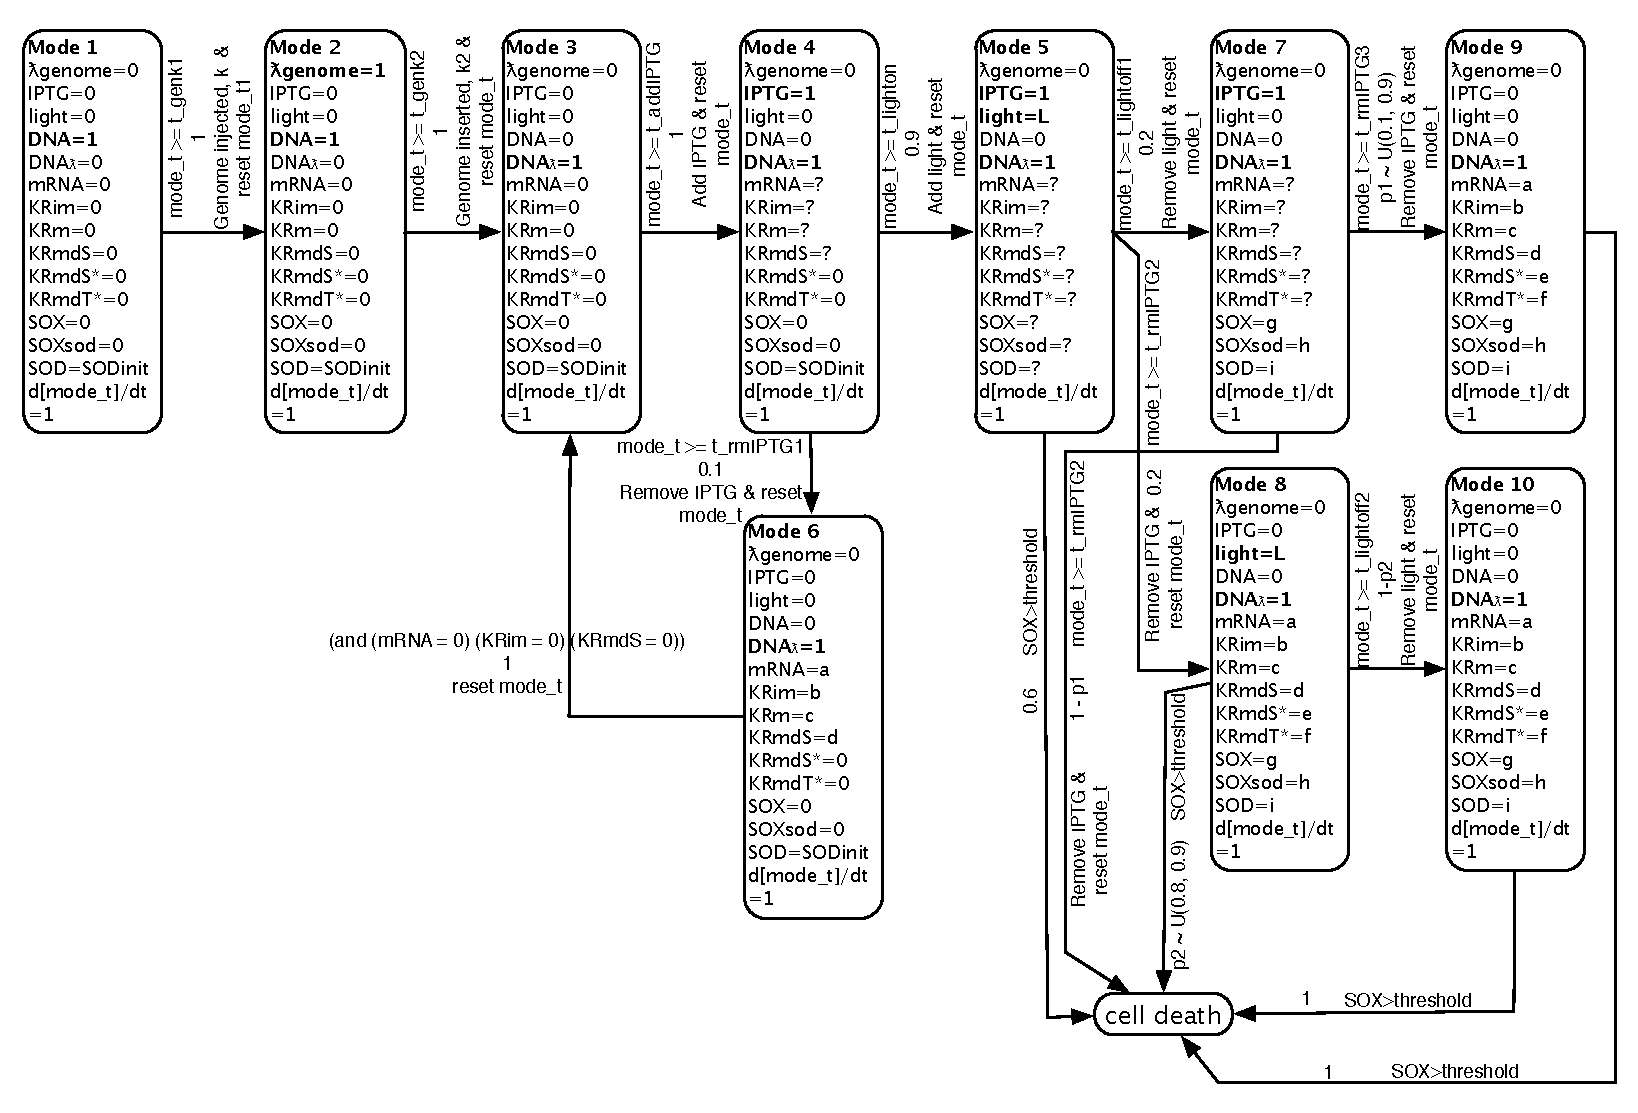
\includegraphics[width=\linewidth]{killerredmodel}
\caption{A probabilistic hybrid automaton for synthesized phage-based therapy model}
\label{fig:killerred}
\end{figure*}

\textbf{\textit{Synthesized Killerred Model.}} The ODEs missing in Figure \ref{fig:killerred} are as follows.
\begin{eqnarray*}
\frac{\mathrm{d}[mRNA]}{\mathrm{d}t} & =& k_{RNAsyn} \cdot [DNA] - k_{RNAdeg} \cdot [mRNA]\\
\frac{\mathrm{d}[KR_{im}]}{\mathrm{d}t} & =& k_{KR_{im}syn} \cdot [mRNA] - (k_{KR_m} + k_{KR_{im}deg})\\
& & \cdot [KR_{im}]\\
\frac{\mathrm{d}[KR_{mdS}]}{\mathrm{d}t} &=& k_{KR_{m}} \cdot [KR_{im}] - k_{KR_{mdS}deg} \cdot [KR_{mdS}]\\
& &(before\; turning \; on \; the \; light)\\
\frac{\mathrm{d}[KR_{mdS}]}{\mathrm{d}t} &=& k_{KR_{m}} \cdot [KR_{im}] + k_{KR_f} \cdot [KR_{mdS^*}] \\
& &+ k_{KR_{ic}} \cdot [KR_{mdS^*}] + k_{KR_{nrd}} \cdot [KR_{mdT^*}]\\
& &+ k_{KR_{SOXd1}} \cdot [KR_{mdT^* }] - k_{KR_{ex}} \cdot [KR_{mdS}]\\
& &- k_{KR_{mdS}deg} \cdot [KR_{mdS}]\;\;\; (after\; adding\; light)\\
\frac{\mathrm{d}[KR_{mdS^*}]}{\mathrm{d}t} &=& k_{KR_{ex}} \cdot [KR_{mdS}] - k_{KR_f } \cdot [KR_{mdS^*}] \\
& &-k_{KR_{ic}} \cdot [KR_{mdS^*}] - k_{KR_{isc}} \cdot [KR_{mdS^*}]\\
& &- k_{KR_{mdS^*}deg} \cdot [KR_{mdS^*}]\\
\frac{\mathrm{d}[KR_{mdT^*}]}{\mathrm{d}t} &=& k_{KR_{isc}} \cdot [KR_{mdS^*}] - k_{KR_{nrd}} \cdot [KR_{mdT^*}]\\
& &- k_{KR_{SOXd1}} \cdot [KR_{mdT^*}]\\
& &- k_{KR_{SOXd2}} \cdot [KR_{mdT^*}]\\
& &- k_{KR_{mdT^*}deg} \cdot [KR_{mdT^*}]
\end{eqnarray*}
\begin{eqnarray*}
\frac{\mathrm{d}[SOX]}{\mathrm{d}t} &=& k_{KR_{SOXd1}} \cdot [KR_{mdT^*}] + k_{KR_{SOXd2}} \cdot [KR_{mdT^*}]\\
& &- \frac{\mathrm{d}[SOX_{sod}]}{\mathrm{d}t}\\
\frac{\mathrm{d}[SOX_{sod}]}{\mathrm{d}t} &=& k_{SOD} \cdot V_{maxSOD} \cdot \frac{[SOX]}{K_m + [SOX]}
\end{eqnarray*}













\section{Experimental results for additional benchmarks}\label{apndx:exp}
\begin{center}
%\begin{sidewaystable}[hp]
\begin{table*}[ht]
\label{table:exp}
\captionsetup{font=scriptsize}
\centering
\begin{tabular}{c|c|c|c|c|c|c|c|c|c|c|c}
\hline
Benchmark & \#Ms & K & \#ODEs & \#Vs & \#RVs & $\delta$ & Est\_P & \#S\_S & \#T\_S & A\_T(s) & T\_T(s) \\ \hline
BBK1 & 1 & 1 & 2 & 14 & 3 & 0.001 & 0.754 & 5372 & 7126 & 0.086 & 612.836 \\ \hline
BBK5 & 1 & 5 & 2 & 38 & 3 & 0.001 & 0.059 & 209 & 3628 & 0.253 & 917.884 \\ \hline
BBwDv1 & 2 & 2 & 4 & 20 & 4 & 0.001 & 0.208 & 2206 & 10919 & 0.080 & 873.522 \\ \hline
BBwDv2K2 & 2 & 2 & 4 & 20 & 3 & 0.001 & 0.845 & 7330 & 8669 & 0.209 & 1811.821 \\ \hline
BBwDv2K8 & 2 & 8 & 4 & 56 & 3 & 0.001 & 0.207 & 2259 & 10901 & 0.858 & 9353.058 \\ \hline
Tld & 2 & 7 & 2 & 33 & 4 & 0.001 & 0.996 & 227 & 227 & 0.213 & 48.351 \\ \hline
Ted & 2 & 7 & 4 & 50 & 4 & 0.001 & 0.996 & 227 & 227 & 12.839 & 2914.448 \\ \hline
DTldK3 & 2 & 3 & 4 & 26 & 2 & 0.001 & 0.996 & 227 & 227 & 0.382 & 86.714 \\ \hline
DTldK5 & 2 & 5 & 4 & 38 & 2 & 0.001 & 0.161 & 1442 & 8961 & 0.280 & 2509.078 \\ \hline
W4mv1 & 4 & 3 & 8 & 26 & 6 & 0.001 & 0.381 & 5953 & 15639 & 0.238 & 3722.082 \\ \hline
W4mv2K3 & 4 & 3 & 8 & 26 & 6 & 0.001 & 0.996 & 227 & 227 & 0.673 & 152.771 \\ \hline
W4mv2K7 & 4 & 7 & 8 & 50 & 6 & 0.001 & 0.004 & 0 & 227 & 0.120 & 27.240 \\ \hline
DWK1 & 2 & 1 & 4 & 14 & 5 & 0.001 & 0.996 & 227 & 227 & 0.171 & 38.817 \\ \hline
DWK3 & 2 & 3 & 4 & 26 & 5 & 0.001 & 0.996 & 227 & 227 & 0.215 & 48.806 \\ \hline
DWK9 & 2 & 9 & 4 & 62 & 5 & 0.001 & 0.996 & 227 & 227 & 5.144 & 1167.688 \\ \hline
Que & 3 & 2 & 3 & 13 & 4 & 0.001 & 0.228 & 2662 & 11677 & 0.095 & 1109.315 \\ \hline
3dOsc & 3 & 2 & 18 & 48 & 2 & 0.001 & 0.996 & 227 & 227 & 8.273 & 1877.969 \\ \hline
QuadC & 1 & 0 & 14 & 44 & 6 & 0.001 & 0.996 & 227 & 227 & 825.641 & 187420.507 \\ \hline
ExPHA01 & 2 & 2 & 4 & 20 & 2 & 0.001 & 0.524 & 345 & 658 & 5.01 & 3295.82 \\ \hline
ExPHA02 &  2  &  3  & 2  & 17 & 1  &  0.001 &  0.900  & 5361 & 5953  & 0.0004   & 2.35  \\ \hline
KRk5 & 6   &  5  & 84  &194  & 2  &  0.001 &  0.544 & 8946   & 16457     &  0.122  & 2015.64  \\ \hline
KRk6 & 8   &  6  &112   &224  &  6 &  0.001 &  0.246  & 2032   & 8263     & 1.385   & 11444.22  \\ \hline
KRk7 & 10   &  7  & 150  &271  & 6  &  0.001 & 0.096 & 558   & 5795     & 16.275   & 94311.18  \\ \hline
KRk8 &  7  &  8  & 105  &303  & 6  &  0.001 &   0.004       &  0  & 227     & 0.003   & 0.58  \\ \hline
KRk9 &  9  &  9  & 135  & 335 & 6  &  0.001 &   0.004       & 0   & 227     & 0.015   &3.43   \\ \hline
KRk10 & 11   &  10  & 165  & 367 & 6  &  0.001 &  0.004        &0   &  227    & 0.026   &  5.92 \\ \hline
\end{tabular}
\caption {\#Ms = number of modes, K indicates the unfolding steps, \#ODEs = number of ODEs in the model, \#Vs = number of total variables in the unfolded formulae, \#RVs = number of random variables in the model, $\delta$ = precision used in {\it dReach}, \#S\_S = number of $\delta$-sat samples , \#T\_S = total number of samples, Est\_P = estimated maximum posterior probability,  A\_T(s) = average CPU time of each sample in seconds, and T\_T(s) = total CPU time for all samples in seconds.}
\label{table:additonalexp}
\end{table*}
%\end{sidewaystable}
\end{center}

\begin{table*}[th!]
\captionsetup{font=scriptsize}
\centering
    \begin{tabular}{|c|c|c|c|c|c|c|c|c|c|c|}
    \hline
    $t_{lighton}$ & 1 & 2 & 3 & 4 & 5 & 6 & 7 & 8 & 9 & 10 \\ \hline
    $t_{tot}$ & 16  & 17.2     &  18.5   & 20   & 21.3 & 22.7 & 23.5 & 24.1 & 25 & 30    \\ \hline
    \end{tabular}
    \caption{The relation between the time to turn on the light after adding IPTG and the total time to kill bacteria cells ($k=5$). }
    \label{table:kr02}
\end{table*}

\begin{table*}[th!]
\captionsetup{font=scriptsize}
\centering
    \begin{tabular}{|c|c|c|c|c|c|c|c|c|c|c|}
    \hline
    $t_{lightoff1}$ & 1 & 2 & 3 & 4 & 5 & 6 & 7 & 8 & 9 & 10 \\ \hline
    $kill bacteria cells$ & Failed  & Failed    &  Failed   & Succ   & Succ & Succ & Succ & Succ & Succ & Succ    \\ \hline
    \end{tabular}
    \caption{The impact of the time duration that the cells are exposed to light ($k=6$).}
    \label{table:kr03}
\end{table*}

The table \ref{table:additonalexp} shows the results of experiments. To further demonstrate the feasibility of {\it SReach}, these experiments were conducted with the sequential version of {\it SReach} on a machine with 2.9GHz Intel Core i7 processor and 8GB RAM, running OS X 10.9.2. In our experiments we used $0.001$ as the precision for the $\delta$-decision problem; and Bayesian sequential estimation with $0.01$ half-interval width, coverage probability $0.99$, and uniform prior ($\alpha = \beta = 1$). In the following table, BB refers to the bouncing ball models, Tld the thermostat model with linear temperature decrease, Ted the thermostat model with exponential decrease, DT the dual thermostat models, W the watertank models, DW the dual watertank models, Que the model for queuing system which has both nonlinear functions and nondeterministic jumps, 3dOsc the model for 3d oscillator, and QuadC the model for quadcopter stabilization control. Following these hybrid systems with parametric uncertainty, we also consider two example PHAs - ExPHA01and EXPHA02, and PHAs with additional randomness - KR our killerred models.



%%%%%%%%%%%%%%%%%%%%
\end{document}
